\documentclass{article}
%\documentclass{article}

\usepackage{tikz}
\usetikzlibrary{external}

\usepackage{braket}

\usepackage{subcaption} % Subfigure environment 
\usepackage{gensymb}

\usepackage{amsmath} % Mathematical symbols
\usepackage{amssymb} % Symbols

\usepackage{caption}% Captions onder figuur gecentreerd
%\usepackage[toc,page]{appendix}
\usepackage{subcaption} % Subfigure environment 
\usepackage{float}

\usepackage{etoolbox} %for if empty functionality

\usepackage{ifthen}

%break long urls at a - and not only at . or /
\usepackage{url}
\def\UrlBreaks{\do\/\do-}
\usepackage{breakurl}
\usepackage[hidelinks,breaklinks]{hyperref}

\usepackage{verbatim}
\usepackage{siunitx} % Elegant eenheden zetten
\usepackage[version=3]{mhchem} % ingeven van chemische fomules
\usepackage{cleveref} % Paragraaf tekens
\usepackage{longtable}
%\usepackage{lscape}
\usepackage[T1]{fontenc}
\usepackage{fontenc}
\usepackage{amsfonts}
\usepackage{mathtools}
\usepackage{grffile}%double dot in figure name
\usepackage{lipsum}
\usepackage{siunitx}
\usepackage{xcolor}
\usepackage{sectsty}
\usepackage{booktabs}
\usepackage{physics}
\usepackage{leftidx}
\usepackage[utf8]{inputenc}
\usepackage{gensymb} % /textdegree


%\setcounter{tocdepth}{4}
\setcounter{secnumdepth}{4}

\usepackage{graphicx}

\usepackage{todonotes}

%\usepackage[nottoc]{tocbibind}

\title{Thesis}

\date{2020}

\begin{document}

%\def\temp{#1}\ifx\temp\empty
%  <EMPTY>%
%\else
%  <NON EMPTY>%
%\fi

\newcommand{\combineTikz}[3]{
    \begin{tikzpicture}[baseline={0-0.5*height("$=$")}]
        \node (AA) at (0,0)  { #1   };
        \node (AB) at ( {#3} ,0)  {  #2  };
    \end{tikzpicture}
}

%\newcommand{\mpo}[6]  {\tikzexternalenable { \begin{tikzpicture}[baseline={0-0.5*height("$=$")}]
\newcommand{\mpo}[6]  { \begin{tikzpicture}[baseline={0-0.5*height("$=$")}]

        %\def \NNodes {#1}
        %\def \NodeName {#2}          
        %\def \NodeName {#2}          
        %\def \NodeName {#2}          
        %\def \NodeName {#2}          
        %\def \NodeName {#2}          
        %\def \NameUp   {#3} 
        %\def \NameUp   {#3} 
        %\def \NameUp   {#3} 
        %\def \NameUp   {#3} 
        %\def \NameUp   {#3} 
        %\def \NameDown  {#4}	
        %\def \NameDown  {#4}	
        %\def \NameDown  {#4}	
        %\def \NameDown  {#4}	
        %\def \NameDown  {#4}	

        \def \legLength {0.7}
        \def \radius {0.3}

        \pgfmathsetmacro{\step}{2*\radius+\legLength}
        \pgfmathsetmacro{\legpos}{\radius+\legLength}

        \pgfmathsetmacro{\Nmax}{#1-1}

        \foreach \N in {0,..., \Nmax }{
                \pgfmathsetmacro{\p}{\N*\step}

                % up and down labels
                \def\temp{#3}\ifx\temp\empty
                    \def \labelUp {}
                \else
                    \pgfmathsetmacro{\labelUp}{  {#3}[\N]  }
                \fi

                \def\tempp{#4}\ifx\tempp\empty
                    \def \labeldown {}
                \else
                    \pgfmathsetmacro{\labeldown}{  {#4}[\N]  }
                \fi

                \def\aab{#5}\ifx\aab\empty
                    \def \dotssite {0}
                \else
                    \pgfmathsetmacro{\dotssite}{  {#5}[\N]  }
                \fi

                \ifthenelse{\dotssite = 0}{

                    \def\aac{#6}\ifx\aac\empty
                        \def \nname {O}
                    \else
                        \pgfmathsetmacro{\nname}{  {#6}[\N]  }
                    \fi

                    \node[circle,draw, radius=\radius] (O\N) at (\p,0) {\nname};

                    \ifthenelse{ \equal{\labelUp}{-}  }{
                    }{
                        \node[] (Ou\N) at (\p, \legpos ) { \labelUp };
                        \draw (O\N) -- (Ou\N);
                    }

                    \ifthenelse{ \equal{\labeldown}{-}  }{
                    }{
                        \node[] (Od\N) at (\p,-\legpos) {\labeldown};
                        \draw (O\N) -- (Od\N);
                    }

                }{
                    \node[circle] (O\N) at (\p,0) { $\cdots$ };
                }

            }

        \ifthenelse{  #1  =1  }{}{
            \foreach \N in {1,...,\Nmax }{
                    \pgfmathsetmacro{\M}{\N-1}
                    \pgfmathsetmacro{\label}{ {#2}[\N]  }
                    %\pgfmathsetmacro{\label}{ 5}

                    \draw (O\M) --  node[above]  {\label} (O\N);
                }
        }

        \pgfmathsetmacro{\labelo}{ {#2}[0]}
        \pgfmathsetmacro{\labeli}{  {#2}[\Nmax+1]}

        \ifthenelse{ \equal{\labelo}{Tr}  }{

            \pgfmathsetmacro{\endpos}{\step*\Nmax+\radius}

            \draw plot [smooth ]  coordinates { (-\radius,0)    (-\radius, -0.45 )  (\endpos, -0.45)   (O\Nmax)   } ;
        }{
            \ifthenelse{ \equal{\labelo}{-}  }{
            }{
                \pgfmathsetmacro{\endpos}{\step*\Nmax+\legpos}

                \node (N0) at (-\legpos,0) {};
                \node (Ne) at (\endpos,0) {};

                \draw (N0) -- node[above] {\labelo} (O0);

                \draw (Ne) -- node[above] {\labeli}  (O\Nmax);
            }
        }
        %\draw (O0) --  node[above] {1} (O1);
        %\end{tikzpicture}} \tikzexternaldisable}
    \end{tikzpicture}}

%\newcommand{\expH}[5]{\tikzexternalenable { \begin{tikzpicture}[baseline={0-0.5*height("$=$")}]
\newcommand{\expH}[5]{\begin{tikzpicture}[baseline={0-0.5*height("$=$")}]
        \def \NNodes {#1};

        \def\aaa{#2}\ifx\aaa\empty
            \def \text { $e^{-\beta \hat{H}_{\NNodes} }$ }
        \else
            \def \text {#2}
        \fi

        \pgfmathwidth{ "\text" }
        \def \textwidth { \pgfmathresult }

        %\pgfmathsetmacro{\text}{width(\text)}

        \def \legLength {0.6}
        \def \radius {0.3} %fix to fit text inside for size 1
        \def \boxHeight {0.4};

        \pgfmathsetmacro{\step}{2*\radius+\legLength}
        \pgfmathsetmacro{\legpos}{\radius+\legLength}
        \pgfmathsetmacro{\dotpos}{\boxHeight+\legLength/2}

        \pgfmathsetmacro{\Nmax}{\NNodes -1}

        \pgfmathsetmacro{\boxsize}{ max ( \textwidth/1cm , \step*\Nmax )   + \radius}

        %\pgfmathsetmacro{\boxsize}{ 5  )}
        %\pgfmathsetlength{\boxsize}{ max( \textwidth,  \boxsize1  )}

        %            \ifthenelse{#1=1}{
        %                \def \left {-0.6}
        %                \def \right {0.6}
        %            }{
        \def \left {-\radius}
        \def \right {\boxsize}
        %            }

        \draw (\left,- \boxHeight ) rectangle (\right, \boxHeight ) [add reference =H] ;

        \node  at (H center) { \text };

        \foreach \N in {0,..., \Nmax }{
                \pgfmathsetmacro{\p}{\N*\step}

                % up and down labels
                \def\temp{#3}\ifx\temp\empty
                    \def \labelUp {}
                \else
                    \pgfmathsetmacro{\labelUp}{  {#3}[\N]  }
                \fi

                \def\tempp{#4}\ifx\tempp\empty
                    \def \labeldown {}
                \else
                    \pgfmathsetmacro{\labeldown}{  {#4}[\N]  }
                \fi

                \node[] (O\N) at (\p,0) {};

                \ifthenelse{ \equal{\labelUp}{...}  }{
                    \node[] (Ou\N) at (\p, \dotpos ) {\labelUp};
                }{
                    \ifthenelse{ \equal{\labelUp}{-}  }{

                    }{
                        \node[] (Ou\N) at (\p, \legpos ) {\labelUp};
                        \draw (Ou\N) --  (Ou\N  |- H north);
                    }
                }

                \ifthenelse{ \equal{\labeldown}{...}  }{
                    \node[] (Od\N) at (\p,-\dotpos ) {\labeldown};
                }{
                    \ifthenelse{ \equal{\labeldown}{-}  }{

                    }{
                        \node[] (Od\N) at (\p,-\legpos) {\labeldown};
                        \draw (Od\N) --  (Od\N  |- H south);
                    }
                }
            }

        \def\tempt{#5}\ifx\tempt\empty

        \else
            \pgfmathsetmacro{\labelo}{ {#5}[0] }
            \pgfmathsetmacro{\labeli}{  {#5}[1] }

            \pgfmathsetmacro{\leftleg}{  \left - \legLength }
            \pgfmathsetmacro{\rightleg}{  \right + \legLength }

            \node (N0) at (\leftleg,0) {\labelo};
            \draw (N0) -- ( N0  -| H west);

            \node (Ne) at (\rightleg,0) {\labeli};
            \draw (Ne) --  ( Ne  -| H east);
        \fi

        %        \end{tikzpicture}} \tikzexternaldisable }
    \end{tikzpicture} }

%\newcommand{\mpob}[6]  {\tikzexternalenable { \begin{tikzpicture}[baseline={0-0.5*height("$=$")},scale=0.8]
\newcommand{\mpob}[6]  {\begin{tikzpicture}[baseline={0-0.5*height("$=$")},scale=0.8]

        %\def \NNodes {#1}
        %\def \NodeName {#2}          
        %\def \NodeName {#2}          
        %\def \NodeName {#2}          
        %\def \NodeName {#2}          
        %\def \NodeName {#2}          
        %\def \NameUp   {#3} 
        %\def \NameUp   {#3} 
        %\def \NameUp   {#3} 
        %\def \NameUp   {#3} 
        %\def \NameUp   {#3} 
        %\def \NameDown  {#4}	
        %\def \NameDown  {#4}	
        %\def \NameDown  {#4}	
        %\def \NameDown  {#4}	
        %\def \NameDown  {#4}	

        \def \legLength {1.0}
        \def \radius {0.1}

        \pgfmathsetmacro{\step}{2*\radius+\legLength}
        \pgfmathsetmacro{\legpos}{\radius+\legLength}

        \pgfmathsetmacro{\Nmax}{#1-1}

        \foreach \N in {0,..., \Nmax }{
                \pgfmathsetmacro{\p}{\N*\step}

                % up and down labels
                \def\temp{#3}\ifx\temp\empty
                    \def \labelUp {}
                \else
                    \pgfmathsetmacro{\labelUp}{  {#3}[\N]  }
                \fi

                \def\tempp{#4}\ifx\tempp\empty
                    \def \labeldown {}
                \else
                    \pgfmathsetmacro{\labeldown}{  {#4}[\N]  }
                \fi

                \def\aab{#5}\ifx\aab\empty
                    \def \dotssite {0}
                \else
                    \pgfmathsetmacro{\dotssite}{  {#5}[\N]  }
                \fi

                \def\aac{#6}\ifx\aac\empty
                    \def \nname { "O" }
                \else
                    \pgfmathsetmacro{\nname}{  {#6}[\N]  }
                \fi

                %\node[] (O\N) at (\p,0) {\nname};
                \node[circle,draw, radius=\radius] (O\N) at (\p,0) {\nname};

            }

        \ifthenelse{  #1  =1  }{}{
            \foreach \N in {1,...,\Nmax }{
                    \pgfmathsetmacro{\M}{\N-1}
                    \pgfmathsetmacro{\label}{ {#2}[\N]  }
                    %\pgfmathsetmacro{\label}{ 5}

                    \draw (O\M) --  node[above]  {\label} (O\N);
                }
        }

        % \pgfmathsetmacro{\labelo}{ {#2}[0]}
        % \pgfmathsetmacro{\labeli}{  {#2}[\Nmax+1]}

        % \node (N0) at (-\legpos,0) {};
        % \draw (N0) -- node[above] {\labelo} (O0);

        % \pgfmathsetmacro{\endpos}{\step*\Nmax+\legpos}

        % \node (Ne) at (\endpos,0) {};
        % \draw (Ne) -- node[above] {\labeli} (O\Nmax);

        %\draw (O0) --  node[above] {1} (O1);

        % \end{tikzpicture}} \tikzexternaldisable}

    \end{tikzpicture}}

% \newcommand{\pepob}[5]  { \tikzexternalenable {\begin{tikzpicture}[baseline={0-0.5*height("$=$")},scale=0.8]
% \newcommand{\pepob}[5]  { \begin{tikzpicture}[baseline={0-0.5*height("$=$")},scale=1,
\newcommand{\pepob}[5]  { \begin{tikzpicture}[
            baseline={([yshift= -2ex ]current bounding box.north)},
            %baseline={0-0.5*height("$=$")},
            scale=1,
            Al/.style = {regular polygon, regular polygon sides=3,
                    draw, fill=white, text width=0.1,
                    inner sep=1mm, outer sep=0mm,
                    shape border rotate=-90},
            Ar/.style = {regular polygon, regular polygon sides=3,
                    draw, fill=white, text width=0.1,
                    inner sep=1mm, outer sep=0mm,
                    shape border rotate=90},
            Acc/.style = {diamond, draw, inner sep=1mm},
            Ac/.style = {rectangle, draw, inner sep=2mm}]

        %\pgfmathsetmacro{\llegLength}{ 0.3 }

        \def \legLength { 0.8}
        \def \radius {0.1}

        %\pgfmathtruncatemacro{\llegLength} { 0.8 }
        %\pgfmathtruncatemacro{\radius} { 0.1 }

        %\pgfmathtruncatemacro{\legLength}{2* \llegLength}
        %\pgfmathtruncatemacro{\lstep}{\radius+ \llegLength}
        %\pgfmathtruncatemacro{\step}{2*\lstep}
        \pgfmathsetmacro{\step}{2*\radius+ \legLength}

        \pgfmathsetmacro{\legpos}{\radius+\legLength}

        \pgfmathsetmacro{\Nmax}{#1-1}
        \pgfmathsetmacro{\Mmax}{#2-1}

        % define positions of different O's

        \setcounter{a}{0}
        %\setcounter{a}{0}

        \foreach \N in {0,..., \Nmax }{

                %\pgfmathtruncatemacro{\a}{\thea}

                \pgfmathsetmacro{\p}{  (\N + \thea) *\step   }
                %\setcounter{b}{0}

                \foreach \M in {0,..., \Mmax }{

                        %\pgfmathsetmacro{\p}{ \pp + \theb *\step   }

                        \pgfmathsetmacro{\k}{   \M   *\step  }

                        \pgfmathtruncatemacro{\s}{\M*(\Nmax+1)+\N   }

                        \pgfmathsetmacro{\nname}{ ""  }

                        \def\aab{#5}\ifx\aab\empty
                            \def \so {0}
                        \else
                            \pgfmathsetmacro{\so}{  {#5}[\s]  }
                        \fi

                        \ifthenelse{\so = 0}{
                            \node[circle,draw, radius=\radius] (O\s) at (\p,\k) {\nname};
                        }

                        \ifthenelse{\so = 2}{
                            \node[draw, Al] (O\s) at (\p,\k) {\nname};
                        }

                        \ifthenelse{\so = 3}{
                            \node[draw, Ar] (O\s) at (\p,\k) {\nname};
                        }

                        \ifthenelse{\so = 4}{
                            \node[draw= none, inner sep=0, outer sep=0 , minimum size=0pt] (O\s) at (\p,\k) {\nname};
                        }

                        \ifthenelse{\so = 6}{
                            \node[draw, Acc] (O\s) at (\p,\k) {\nname};
                        }

                        \ifthenelse{\so = 7}{
                            \node[draw, Ac] (O\s) at (\p,\k) {\nname};
                        }

                        %Gl environment
                        \ifthenelse{\so = 5}{

                            \pgfmathsetmacro{\recl}{  \p + \step - 3*\radius  }
                            \pgfmathsetmacro{\recr}{  \p + \step + 3*\radius  }

                            \pgfmathsetmacro{\recu}{  \k + 2*\radius }
                            \pgfmathsetmacro{\recd}{  \k - \step -2*\radius  }

                            % \pgfmathsetmacro{\recl}{  \p  +\step   }
                            % \pgfmathsetmacro{\mw}{ 2*\radius }
                            % \pgfmathsetmacro{\mh}{ \step  }

                            % \pgfmathsetmacro{\recu}{  \k - \step /2 }

                            % \node[rectangle,
                            %     draw,
                            %     minimum height= 1,
                            %     anchor=center  ] (O\s) at (\recl,\recu) {Gl};

                            \draw  (\recl,\recu) rectangle node[  ] (O\s)  {Gl}   (\recr,\recd)     ;

                            %\draw node[fill, minimum width= 1  ,minimum height= 1 ] (O\s) at (\recl,\recu) {Gl};
                            \stepcounter{a}
                        }

                        \ifthenelse{\so = 8}{

                            \node[draw, Ar] (O\s) at (\p,\k) {\nname};

                            \pgfmathtruncatemacro{\t}{\M*(\Nmax+1)+\N +1  }

                            \pgfmathsetmacro{\recl}{  \p +\step  - 3*\radius  }
                            \pgfmathsetmacro{\recr}{  \p + \step+  3*\radius  }

                            \pgfmathsetmacro{\recu}{  \k + 2*\radius }
                            \pgfmathsetmacro{\recd}{  \k - \step -2*\radius  }

                            \draw  (\recl,\recu) rectangle node (O\t)  {Gr}   (\recr,\recd)     ;

                            \draw  (O\s) -- (   O\t.west   |-  O\s  ) ;
                            \stepcounter{a}
                        }

                        \ifthenelse{\so = 9}{

                            \node[draw, Ac] (O\s) at (\p,\k) {\nname};

                            \pgfmathtruncatemacro{\t}{\M*(\Nmax+1)+\N +1  }

                            \pgfmathsetmacro{\recl}{  \p +\step  - 3*\radius  }
                            \pgfmathsetmacro{\recr}{  \p + \step+  3*\radius  }

                            \pgfmathsetmacro{\recu}{  \k + 2*\radius }
                            \pgfmathsetmacro{\recd}{  \k - \step -2*\radius  }

                            \draw  (\recl,\recu) rectangle node (O\t)  {Gr}   (\recr,\recd)     ;

                            \draw  (O\s) -- (   O\t.west   |-  O\s  ) ;
                            \stepcounter{a}
                        }

                        \ifthenelse{\so = 10}{

                            \node[draw = none] (O\s) at (\p,\k) {\nname};

                            \pgfmathtruncatemacro{\t}{\M*(\Nmax+1)+\N +1  }

                            \pgfmathsetmacro{\recl}{  \p +\step  - 3*\radius  }
                            \pgfmathsetmacro{\recr}{  \p + \step+  3*\radius  }

                            \pgfmathsetmacro{\recu}{  \k + 2*\radius }
                            \pgfmathsetmacro{\recd}{  \k - \step -2*\radius  }

                            \draw  (\recl,\recu) rectangle node (O\t)  {Gr}   (\recr,\recd)     ;

                            \draw  (O\s) -- (   O\t.west   |-  O\s  ) ;
                            \stepcounter{a}
                        }

                        \ifthenelse{\so = 11}{

                            \node[draw , Acc] (O\s) at (\p,\k) {\nname};

                            \pgfmathtruncatemacro{\t}{\M*(\Nmax+1)+\N +1  }

                            \pgfmathsetmacro{\recl}{  \p +\step  - 3*\radius  }
                            \pgfmathsetmacro{\recr}{  \p + \step+  3*\radius  }

                            \pgfmathsetmacro{\recu}{  \k + 2*\radius }
                            \pgfmathsetmacro{\recd}{  \k - \step -2*\radius  }

                            \draw  (\recl,\recu) rectangle node (O\t)  {Gr}   (\recr,\recd)     ;

                            \draw  (O\s) -- (   O\t.west   |-  O\s  ) ;
                            \stepcounter{a}
                        }

                        \ifthenelse{\so = 12}{

                            \node[circle,draw, radius=\radius] (O\s) at (\p,\k) {\nname};

                            \pgfmathsetmacro{\pp}{   \p+\legLength/2 }
                            \pgfmathsetmacro{\pm}{   \p-\legLength/2  }

                            \pgfmathsetmacro{\kp}{   \k+\legLength/2  }
                            \pgfmathsetmacro{\km}{   \k-\legLength/2  }

                            \node (Op\s) at (\pp,\kp) {i};
                            \node (Om\s) at (\pm,\km) {j};

                            \draw (O\s.center)  --  (Op\s);
                            \draw  (Om\s) --  (O\s);
                        }

                        \ifthenelse{\so = 13}{

                            \node[draw= none] (O\s) at (\p,\k) { ... };
                        }

                        \ifthenelse{\so = 14}{

                            \node[circle,draw, radius=\radius] (O\s) at (\p,\k) {\nname};

                            \pgfmathsetmacro{\pp}{   \p+\legLength/2 }
                            \pgfmathsetmacro{\pm}{   \p-\legLength/2  }

                            \pgfmathsetmacro{\kp}{   \k+\legLength/2  }
                            \pgfmathsetmacro{\km}{   \k-\legLength/2  }

                            \node (Op\s) at (\pp,\kp) {};
                            \node (Om\s) at (\pm,\km) {};

                            \draw (O\s.center)  --  (Op\s);
                            \draw  (Om\s) --  (O\s);
                        }

                        \ifthenelse{\so = 15}{

                            \node[circle,draw, radius=\radius] (O\s) at (\p,\k) {\nname};

                            \pgfmathsetmacro{\pp}{   \p+\legLength/2 }

                            \pgfmathsetmacro{\kp}{   \k+\legLength/2  }

                            \node (Op\s) at (\pp,\kp) {};

                            \draw (O\s.center)  --  (Op\s);
                        }

                        \ifthenelse{\so = 16}{
                            \node[draw, Ac] (O\s) at (\p,\k) {B};
                        }

                        \ifthenelse{\so = 17}{
                            \node[circle,draw=none, radius=\radius] (O\s) at (\p,\k) {\nname};
                        }

                        \ifthenelse{\so = 18}{

                            \node[circle,draw=none, radius=\radius] (O\s) at (\p,\k) {\nname};

                            \pgfmathtruncatemacro{\t}{\M*(\Nmax+1)+\N +1  }

                            \pgfmathsetmacro{\recl}{  \p +\step  - 3*\radius  }
                            \pgfmathsetmacro{\recr}{  \p + \step+  3*\radius  }

                            \pgfmathsetmacro{\recu}{  \k + 2*\radius }
                            \pgfmathsetmacro{\recd}{  \k - \step -2*\radius  }

                            \draw  (\recl,\recu) rectangle node (O\t)  {Gr}   (\recr,\recd)     ;

                            \draw  (O\s) -- (   O\t.west   |-  O\s  ) ;
                            \stepcounter{a}
                        }

                        \ifthenelse{\so = 22}{
                            \node[draw,line width=0.6mm  ,Al] (O\s) at (\p,\k) {};
                        }

                        \ifthenelse{\so = 23}{
                            \node[draw,line width=0.6mm  ,Ar] (O\s) at (\p,\k) {};
                        }

                        \ifthenelse{\so = 25}{
                            \node[draw,line width=0.6mm ,Ac] (O\s) at (\p,\k) {};
                        }

                        \ifthenelse{\so = 24}{
                            \node[draw, Ac] (O\s) at (\p,\k) {Fl};
                        }

                        \ifthenelse{\so = 26}{
                            \node[draw, Ac] (O\s) at (\p,\k) {Fr};
                        }

                    }
            }

        %connect nodes horizontally with correct name
        \foreach \M in {0,..., \Mmax }{
                \foreach \N in {1,...,\Nmax}{

                        \pgfmathtruncatemacro{\s}{\M*(\Nmax+1)+\N   }

                        \pgfmathtruncatemacro{\t}{\M*(\Nmax+1)+\N  -1 }

                        \pgfmathtruncatemacro{\l}{\M*(\Nmax)+\N -1 }

                        %\pgfmathsetmacro{\label}{ {#2}[\N]  }
                        %\pgfmathsetmacro{\label}{ \l }
                        \pgfmathsetmacro{\label}{ {#3}[\l]  }

                        \def\aab{#5}\ifx\aab\empty
                            \def \so {0}
                        \else
                            \pgfmathsetmacro{\so}{  {#5}[\s]  }
                        \fi

                        \def\aab{#5}\ifx\aab\empty
                            \def \to {0}
                        \else
                            \pgfmathsetmacro{\to}{  {#5}[\t]  }
                        \fi

                        \ifthenelse{ \equal{\label}{Gl}  }{

                            \pgfmathtruncatemacro{\ogl}{ (\M+1)*(\Nmax+1)+\N -1 }

                            \draw (O\ogl.east   |- O\s  )  --  (O\s);

                            \draw (O\t)  --  ( O\ogl.west    |-  O\t  );

                        }{

                            \ifthenelse{ \equal{\label}{Gr}  }{

                                \pgfmathtruncatemacro{\ogl}{ (\M+1)*(\Nmax+1)+\N  }

                                \draw (O\t)  --  ( O\ogl.west    |-  O\t  );

                                \draw (O\ogl.east   |- O\s  )  --  (O\s);

                            }{

                                \ifthenelse{ \NOT  \so = 1  }{
                                    \ifthenelse{ \NOT  \to = 1}{
                                        \ifthenelse{ \equal{\label}{-} }{

                                        }
                                        {

                                            \draw ( O\t.east |- O\s )  --  node[above]  {\label} (O\s);
                                        }
                                    }
                                }
                            }

                        }

                    }
            }

        %connect nodes vertically with correct name
        \foreach \N in {0,...,\Nmax }{
                \foreach \M in {1,..., \Mmax }{

                        \pgfmathtruncatemacro{\s}{\M*(\Nmax+1)+\N   }

                        \pgfmathtruncatemacro{\t}{ (\M-1)*(\Nmax+1)+\N  }

                        \pgfmathtruncatemacro{\l}{\N*\Mmax+\M  -1 }

                        %\pgfmathsetmacro{\label}{ {#4}[\l]  }
                        \pgfmathsetmacro{\label}{ {#4}[\l]  }

                        \def\aab{#5}\ifx\aab\empty
                            \def \so {0}
                        \else
                            \pgfmathsetmacro{\so}{  {#5}[\s]  }
                        \fi

                        \def\aab{#5}\ifx\aab\empty
                            \def \to {0}
                        \else
                            \pgfmathsetmacro{\to}{  {#5}[\t]  }
                        \fi

                        % \pgfmathtruncatemacro{\st}{ \so+\to  }

                        % \ifthenelse{\st = 0}{
                        %     \draw (O\t) --  node[left]  {\label} (O\s);
                        % }

                        \ifthenelse{ \( \NOT  \so = 1 \) \AND \( \NOT  \so = 5 \) }{
                            \ifthenelse{ \NOT  \to = 1}{
                                \ifthenelse{ \equal{\label}{-} }{

                                }
                                {
                                    \draw (O\t) --  node[left]  {\label} (O\s);
                                }
                            }
                        }

                    }
            }

        % \pgfmathsetmacro{\labelo}{ {#2}[0]}
        % \pgfmathsetmacro{\labeli}{  {#2}[\Nmax+1]}

        % \node (N0) at (-\legpos,0) {};
        % \draw (N0) -- node[above] {\labelo} (O0);

        % \pgfmathsetmacro{\endpos}{\step*\Nmax+\legpos}

        % \node (Ne) at (\endpos,0) {};
        % \draw (Ne) -- node[above] {\labeli} (O\Nmax);

        %\draw (O0) --  node[above] {1} (O1);

        % \pgfmathsetmacro{\s}{\Nmax*\step+0.5}
        % \pgfmathsetmacro{\t}{\Mmax*\step+0.5}

        % \draw[draw=none] (-0.5,-0.5) |- (\s,\t) |- cycle;

        %\end{tikzpicture}} \tikzexternaldisable}
    \end{tikzpicture}}



\onecolumn
\begin{titlepage}
    \begin{center}

        \pagenumbering{gobble}
        
\includegraphics[width=4cm]{Figuren/UGent.png} \\[0.5cm]    %Logo UGENT	

        \Large{\textsc{Master Engineering Physics}} \\[0.5cm]  %Vakgroep	

        \normalsize{Year 2020-2021} \\[3cm]  %Academiejaar

        \huge{\textsc{Master desertation}} \\[0.25cm]   %Titel

        \Large{\textsc{Thesis Tensor networks}}\\[0.25cm]

        \large \textnormal{October 2020} \\[2.5cm]   %Extra informatie

        %\small      %Namen

        David Devoogdt \\       [2.5cm]

        Academic supervisor: prof.

        \vfill

    \end{center}
\end{titlepage}

\tableofcontents

\newpage
\listoftodos
\newpage

%\twocolumn
\pagenumbering{arabic}

\tikzset{add reference/.style={insert path={%
                    coordinate [pos=0,xshift=-0.5\pgflinewidth,yshift=-0.5\pgflinewidth] (#1 south west)
                    coordinate [pos=1,xshift=0.5\pgflinewidth,yshift=0.5\pgflinewidth]   (#1 north east)
                    coordinate [pos=.5] (#1 center)
                    (#1 south west |- #1 north east)     coordinate (#1 north west)
                    (#1 center     |- #1 north east)     coordinate (#1 north)
                    (#1 center     |- #1 south west)     coordinate (#1 south)
                    (#1 south west -| #1 north east)     coordinate (#1 south east)
                    (#1 center     -| #1 south west)     coordinate (#1 west)
                    (#1 center     -| #1 north east)     coordinate (#1 east)
                }}}

\section{Introduction}
\todo{write this}

To deal with these strongly correlated systems, a class of methods called tensor networs were introced.

The Hilbert space grows exponentially with system size.

Want to be able to model various Hamiltonians (e.g. Bosons and
Fermions).
Want to avoid the sign problem of quantum Monte Carlo.
Want to measure physical properties and observables

\subsection{Quantum monte carlo}

\section{tensor networks}

\subsection{Graphical notation}

Before explaing tensor networks, some graphical notation should be introduced. This really is a way to conveniently write vectors, matrices an in general tensors without the need to introduce many labels. A tensor T is represented by a circle with a number of external legs, according to the number of external indices. Connected legs are summed. Some examples are shown in \cref{tab:grafical_not}. Every leg which is connected to multiple tensors, is contracted.

\begin{table}[]
    \centering
    \caption{Caption}
    \begin{tabular}{l|l|l}
        conventional            & Einstein                & tensor notation           \\
        \hline
        $\Vec{x}$               & $x_{\alpha}$            &

        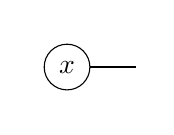
\begin{tikzpicture}[baseline=({N2.base}) ]
            \clip (-0.5,-0.5) rectangle (1,0.5);
            \node[circle, draw] (N2) at (0,0) {$x$};
            \node[] (N1) at (1,0) {};
            \draw  (N1) -- (N2) ;
        \end{tikzpicture}                                                     \\
        M                       & $M_{\alpha \beta}$      & 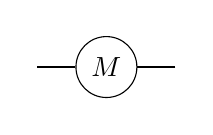
\begin{tikzpicture}[baseline={0cm-0.5*height("$=$")} ]
            \clip (-1,-0.5) rectangle (1,0.5);

            \node[circle, draw] (N2) at (0,0) {$M$};
            \node[] (N0) at (-1,0) {};
            \node[] (N1) at (1,0) {};

            \draw  (N1) -- (N2) ;
            \draw  (N0) -- (N2) ;

        \end{tikzpicture} \\

        $\Vec{x} \cdot \Vec{y}$ & $x_{\alpha} y_{\alpha}$ & 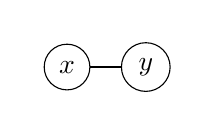
\begin{tikzpicture}[baseline=({N2.base}) ]
            \clip (-0.5,-0.5) rectangle (1.5,0.5);
            \node[circle, draw] (N2) at (0,0) {$x$};
            \node[circle, draw] (N1) at (1,0) {$y$};
            \draw  (N1) -- (N2) ;
        \end{tikzpicture} \\
    \end{tabular}

    \label{tab:grafical_not}
\end{table}

\subsection{Representing a quantum state}

Tensor network come in many shapes and forms. Tensor networks are really used to represent a tensor with many legs. A general quantum state with N sites can be described in a given basis $\ket{i}$ in the following way:
\begin{equation}
    \ket{\Psi} = \sum_{i_1 i_2 \cdots i_n } C^{i_1 i_2 \cdots i_n} \ket{i_1} \otimes \ket{i_2} \otimes \cdots \otimes \ket{i_n}
\end{equation}
Here the tensor $C$ holds all the information of the quantum state. The graphical representation can be seen in \cref{fig:tens:intro:C}.
\begin{figure}
    \centering

    \begin{tikzpicture}[ ]

        \draw (-3,-0) rectangle (1,1)  [add reference=C]   ;
        \node  at (C center) {C};

        \node (N1)  at  (-2.5,-1) {};
        \node (N2)  at  (-1.5,-1) {};
        \node  at  (-.5,-0.5) {...};
        \node  (N3) at  (.5,-1) {};

        \draw    (N1) -- (N1 |-  C south);
        \draw    (N2) -- (N2 |-  C south);
        \draw    (N3) -- (N3 |-  C south);

    \end{tikzpicture}

    \caption{Caption}
    \label{fig:tens:intro:C}
\end{figure}

This requires an exponential number $d^n$ of coefficients C where d is the dimensions of basis $\ket{i}$. In order to make the problem tractable, the following form is proposed as wave function:
\begin{equation}
    C^{i_1 i_2 \cdots i_n} = {C^{1}}_{\alpha_1}^{ i_1} {C^{2}}_{\alpha_1 \alpha_2}^{i_2} \cdots  {C^{n}}_{\alpha_{n-1} }^{i_n}
\end{equation}

\begin{equation}
    \mpo{4}{{"-",,,,,}}{{"$i_1$","$i_2$",,"$i_n$","-"}}{{"-","-",,"-","-"}}{{0,0,1,0,0}}{{"$C^1$", "$C^2$",,"$C^n$", }}
\end{equation}

Where summation over shared indices is implied. It is always possible to find such a representation by means of matrix decomposition (see \cref{sec:mpomath}). The summation over $\alpha_i$ are called a virtual bond and their dimension is denoted by $\chi$. At this point, this is not yet an improvement because the bond dimension needs to be exponentially large in order to represent the tensor C exactly.

Explicit translational invariance is given by tensor $C^i_{\alpha \beta }$ that don't depend on the location. The chain is closed by a matrix M which contains the boundary condiditions. Setting $\alpha_n = \alpha_0$. We can now write this as a Trace over matrix products:

\begin{equation}
    \ket{\Psi} = \Tr( C^{i_1} C^{i_2} \cdots C^{i_n} M  ) \ket{i_1} \otimes \ket{i_2} \otimes \cdots \otimes \ket{i_n}
\end{equation}

\begin{equation}
    \mpo{5}{{"Tr",,,,,}}{{"$i_1$","$i_2$",,"$i_n$","-"}}{{"-","-",,"-","-"}}{{0,0,1,0,0}}{{"C", "C",,"C","M" }}
\end{equation}

\subsection{Classification}

\subsubsection{MPS}

\paragraph{MPO}

Similarly, a Matrix Product Operator (MPO) is of the following form:

\begin{equation} \label{def_mpo}
    \begin{split}
        \hat{O} &= \sum Tr(A^{i_1 j_1} A^{i_2 j_2} \cdots A^{i_n j_n} M) \\
        & \times \ket{i_1}\bra{j_1} \otimes \ket{i_2}\bra{j_2} \otimes \cdots \otimes \ket{i_n}\bra{j_n}
    \end{split}
\end{equation}

\mpo{5}{{"Tr",,,,,}}{{"$i_1$","$i_2$",,"$i_n$","-"}}{{"$j_1$","$j_2$",,"$j_n$","-"}}{{0,0,1,0,0}}{{"A", "A",,"A","M" }}

The matrix M contains the boundary conditions of the operator. Many Hamiltonians can be represented by an MPO. For ins

\paragraph{PEPS}

%https://arxiv.org/pdf/1306.2164.pdf
Exact contraction is hashtag P-Hard:

No exact canonical form

\paragraph{PEPO}

\paragraph{Others}

MERA,TTN,

\todo{ ather tns }

%https://link.springer.com/content/pdf/10.1007%2F978-3-030-34489-4.pdf

\section{Operator exponentials}

\subsection{Statistical mechanics}

The physics of a system in thermodynamical equilibrium can be derived from it's partition function Z.
\begin{equation}
    \begin{split}
        Z &= \sum e^{ - \beta E_n} \\
        &= \sum_n \Braket{n | e^{ - \beta \hat{H} }  | n} \\
        &= \Tr( e^{ - \beta \hat{H} } )
    \end{split}
\end{equation}
The first line is the partition function for clasical discrete systems. The index n runs of all possible microstates. It is know that the propability to find the system in a given microstates is given by:
\begin{equation}
    p_i = \frac{\sum e^{ - \beta E_i}}{Z}
\end{equation}
An useful quantity is the density matrix $\rho$.
\begin{equation}
    \begin{split}
        \rho &= \sum_j p_i  \Ket{ \Psi_j} \Bra{\Psi_j}   \\
        &= \sum_j \frac{ e^{ - \beta \hat{H} } }{Z}  \Ket{ \Psi_j} \Bra{\Psi_j}
    \end{split}
\end{equation}
With this notation
\begin{equation}
    \begin{split}
        Z &= \Tr( \rho) \\
        \Braket{X} &= \Tr(\rho \hat{X})
    \end{split}
\end{equation}

\subsection{Time evolutions}

\subsection{Tensor network methods}

% https://arxiv.org/pdf/1901.05824.pdf

\subsubsection{Approximations to  \texorpdfstring{$ \hat{U}(\delta)$}{U}   }

TEBD, MPO $W^{I,II}$

\subsubsection{global Krylov method }

\subsubsection{MPS-local methods }
local Krylov
TDVP

\section{Tensor network manipulations}
This section serves as an introduction of tensor network manipulations. The overview mainly focusses on MPS/MPO networks, but most of the oprations translate to the 2D case.

The MPS's are processed by transforming the tensor into a matrix, performing some matrix calculations and casting it back into its original form. In this way, the standard methods from linear algebra can be used. This section gives some examples how this is done in practice:

\subsection{Basics}

\subsubsection{Grouping legs}
One of the most basic manipulations is to group some legs of a tensor into one leg:
\begin{equation}
    \begin{split}
        T^{i_1 i_2 j_1 j_2} &=  \expH{2}{$T$}{{"$i_1$","$i_2$"}}{{"$j_1$","$j_1$"}}{} \\
        & \cong \expH{2}{$T$}{{"-","-"}}{{"-","-"}}{{"$(i_1 j_1 )$","$(i_2 j_2)$"}} \\
        &= T^{ (i_1 j_1 ) (i_2 j_2) } \\
    \end{split}
\end{equation}
The dimension of the new leg is the product of the dimension of the individual legs. Contracting 2 merged legs with 2 merged legs is exactly the same as contracting them separately. The both The 4 leg tensor and matrix contain exactly the same information.
Manipulating this in memory requires both permute and reshape commands. This requires some time, the internal representation of the matrix changes.

\subsubsection{decomposition} \label{decompMPO}

The grouping above can be applied to decompose a tensor into 2 tensor with matrix techniques. An example, which will be needed later on, is give here.

\def \figone {\expH{2}{$O^{u v,v w}$}{{"$i_1$","$i_2$"}}{{"$j_1$","$j_1$"}}{{"u","w"}}}

\begin{equation}
    \begin{split}
        \figone &= O^{i_1 i_2 j_1 j_2 }_{\alpha_u \gamma_w} \\
        &\cong O^{u w}_{ (\alpha_u i_1 j_1) (\gamma_w i_2 j_2) } \\
        &= O^{u v}_{(\alpha_u i_1 j_1) \alpha_v } O^{v w}_{ \alpha_v (\alpha_w i_2 j_2) } \\
        &\cong \mpo{2}{{"u","v","w"}}{{"$i_1$","$i_2$"}}{{"$j_1$","$j_1$"}}{}{}
    \end{split}
\end{equation}

The indices U,V and W represent blocks indices. Step 2 reshapes and groups the indices on to one index on the left and one on the right. The dimension of this index is the product of the separate dimensions. Step 3 decomposes the matrix into a product of 2 matrices. The last step transforms the indices back to separate legs.

For an exact representation, the bond dimension of virtual level v is:
\begin{equation}
    \dim{v} = \min( \dim{u}, \dim{v}) + 2 \dim{i}
\end{equation}

Many matrix decompositions exist. Some useful examples here are SVD decomposition, eigenvalue decomposition, QR, $\cdots$.

\subsubsection{virtual levels}
In the previous example, the levels were indicate with a block index or virtual level. The idea is to create seperate the contraction into blocks. This is completely analogous to matrix block multipliction. This wil be a more natural form to represent the algorithm. Of course, one can easily switch between block representation and the full one.

\subsubsection{inverse}
Suppose we want to find a MPO O for given tensors A and B such that the following holds:

\def \figone {\expH{2}{$A$}{{"$i_1$","$i_2$"}}{{"$j_1$","$j_2$"}}{{"u",}}}
\def \figthree {\expH{3}{$B$}{{"$i_1$","$i_2$","$i_3$"}}{{"$j_1$","$j_2$","$j_3$"}}{{"u","v"}}}

\def \figtwo {\mpo{1}{{,"v"}}{{"$i_3$",}}{{"$j_3$",}}{}{}}

\begin{equation}
    \combineTikz{ \figone }{\figtwo}{1.8} =  \figthree
\end{equation}

Again, the indices can be taken toghether in the following way: $\alpha = (u i_1 j_1  i_2 j_2)$ and $\beta = (i_3 j_3 v)$:
\begin{equation}
    A_{\alpha \gamma} O_{\gamma \beta} = B_{\alpha \beta}
\end{equation}
This a a standard matrix equation and can hence be solved with linear algebra packages. Note that it is not necessary to calculate $A^{-1}$ to obtain the solution. Linear solver are generally much faster. As this is one of the core problems to solve both in 1D and 2D, this will be discussed in detail in \cref{sec:framework_impl}.

\subsubsection{contraction order}

\todo{contraction order}

\subsubsection{Gauge freedom}

\todo{gauge}
\subsubsection{truncation}

\todo{svd truncation}

\subsection{MPS algoritms}

%https://arxiv.org/pdf/1306.2164.pdf

\subsubsection{cononical form}

schmidt decomp,

\subsubsection{DMRG}

\subsubsection{Expectation values}

Suppose that the there is an MPO representation of $ e^{ - \beta \hat{H} } $ A and that the mpo represenation for X Y is localised over n sites, then the expactation value is given by:

\begin{equation}
    \Braket{X} = \frac{
        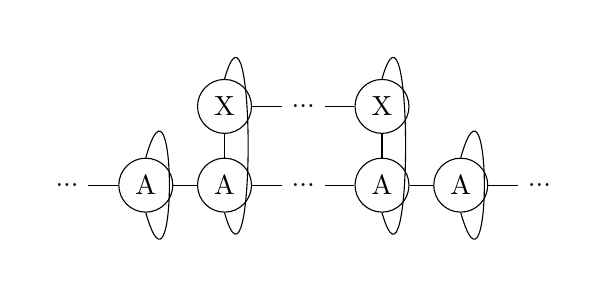
\begin{tikzpicture} [   ]
            \clip (-1.5,-1) rectangle (5.5,2);

            \node[] (N0) at (-1,0) {...};
            \node[circle, draw] (N1) at (0,0) {A};
            \node[circle, draw] (N2) at (1,0) {A};
            \node[circle, draw] (X2) at (1,1) {X};

            \node[] (N3) at (2 ,0) {...};
            \node[] (X3) at (2,1) {...};

            \node[circle, draw] (N4) at (3 ,0) {A};
            \node[circle, draw] (X4) at (3,1) {X};

            \node[circle, draw] (N5) at (4 ,0) {A};
            \node[] (N6) at (5 ,0) {...};

            \draw  (N0) -- (N1) ;

            \draw  (N1) -- (N2) ;
            \draw  (N2) -- (N3) ;
            \draw  (N3) -- (N4) ;
            \draw  (N4) -- (N5) ;
            \draw  (N5) -- (N6) ;

            \draw  (X2) -- (X3) ;
            \draw  (X3) -- (X4) ;

            \draw  (N2) -- (X2) ;
            \draw  (N4) -- (X4) ;

            \draw (X2.north)   .. controls +(0.4,1.4) and +(0.4,-1.4) .. (N2.south);
            \draw (X4.north)   .. controls +(0.4,1.4) and +(0.4,-1.4) .. (N4.south);

            \draw (N1.north)   .. controls +(0.4,1.4) and +(0.4,-1.4) .. (N1.south);
            \draw (N5.north)   ..  controls +(0.4,1.4) and +(0.4,-1.4)  .. (N5.south);
        \end{tikzpicture}
    }{
        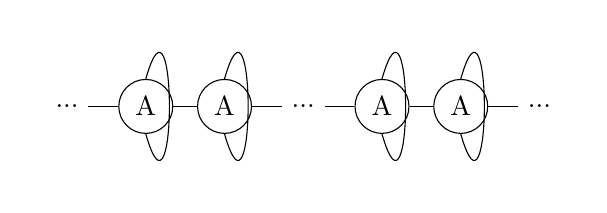
\begin{tikzpicture} [   ]

            \clip  (-1.5,-3) rectangle (5.5,-1);

            \node[] (O0) at (-1,-2) {...};
            \node[circle, draw] (O1) at (0,-2) {A};
            \node[circle, draw] (O2) at (1,-2) {A};

            \node[] (O3) at (2 ,-2) {...};
            \node[circle, draw] (O4) at (3 ,-2) {A};

            \node[circle, draw] (O5) at (4 ,-2) {A};
            \node[] (O6) at (5 ,-2) {...};

            \draw  (O0) -- (O1) ;

            \draw  (O1) -- (O2) ;
            \draw  (O2) -- (O3) ;
            \draw  (O3) -- (O4) ;
            \draw  (O4) -- (O5) ;
            \draw  (O5) -- (O6) ;

            \draw (O2.north)   .. controls +(0.4,1.4) and +(0.4,-1.4) .. (O2.south);
            \draw (O4.north)   .. controls +(0.4,1.4) and +(0.4,-1.4) .. (O4.south);

            \draw (O1.north)   .. controls +(0.4,1.4) and +(0.4,-1.4) .. (O1.south);
            \draw (O5.north)   ..  controls +(0.4,1.4) and +(0.4,-1.4)  .. (O5.south);
        \end{tikzpicture}
    }
    \label{sm:expecatation_X}
\end{equation}

In the thermodynamic limit there are an infinity number of A to the left and the right. This can be simulated by taking the left and right fixed points of the traced MPO A corresponding to the largest eigenvector $\lambda$.

\begin{equation}
    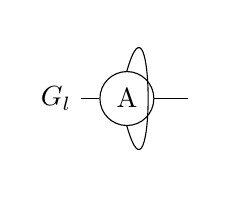
\begin{tikzpicture}[baseline={0cm-0.5*height("$=$")} , scale=0.9]
        \clip (-1.4,-1) rectangle (1,1);
        \node[] (N0) at (-1,0) {$G_l$};
        \node[] (N2) at (1,0) {};
        \node[circle, draw] (N1) at (0,0) {A};
        \draw  (N0) -- (N1) ;
        \draw  (N1) -- (N2) ;
        \draw (N1.north)   .. controls +(0.4,1.4) and +(0.4,-1.4) .. (N1.south);
    \end{tikzpicture}
    = \lambda
    \begin{tikzpicture}[baseline={0cm-0.5*height("$=$")}, scale=0.9 ]
        \clip (-.4,0.5) rectangle (1,-0.5);
        \node[] (N2) at (1,0) {};
        \node[] (N1) at (0,0) {$G_l$};
        \draw  (N1) -- (N2) ;
    \end{tikzpicture}
\end{equation}

\begin{equation}
    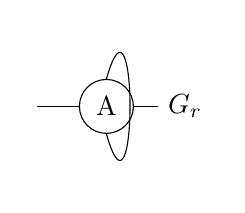
\begin{tikzpicture}[baseline={0cm-0.5*height("$=$")} ]
        \clip (-1,-1) rectangle (1.4,1);
        \node[] (N0) at (-1,0) {};
        \node[] (N2) at (1,0) {$G_r$};
        \node[circle, draw] (N1) at (0,0) {A};
        \draw  (N0) -- (N1) ;
        \draw  (N1) -- (N2) ;
        \draw (N1.north)   .. controls +(0.4,1.4) and +(0.4,-1.4) .. (N1.south);
    \end{tikzpicture}
    = \lambda
    \begin{tikzpicture}[baseline={0cm-0.5*height("$=$")} ]
        \clip (0,-0.5) rectangle (1.4,0.5);
        \node[] (N2) at (1,0) {$G_l$};
        \node[] (N1) at (0,0) {};
        \draw  (N1) -- (N2) ;
    \end{tikzpicture}
\end{equation}

Equation \cref{sm:expecatation_X} can now be easily caclulated:

\begin{equation}
    \Braket{X} = \frac{
        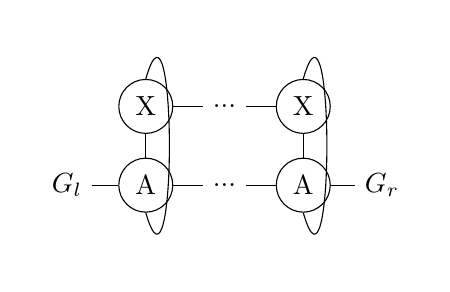
\begin{tikzpicture} [   ]
            \clip (-0.5,-1) rectangle (4.5,2);

            \node[] (N1) at (0,0) {$G_l$};
            \node[circle, draw] (N2) at (1,0) {A};
            \node[circle, draw] (X2) at (1,1) {X};

            \node[] (N3) at (2 ,0) {...};
            \node[] (X3) at (2,1) {...};

            \node[circle, draw] (N4) at (3 ,0) {A};
            \node[circle, draw] (X4) at (3,1) {X};

            \node[] (N5) at (4 ,0) {$G_r$};

            \draw  (N1) -- (N2) ;
            \draw  (N2) -- (N3) ;
            \draw  (N3) -- (N4) ;
            \draw  (N4) -- (N5) ;

            \draw  (X2) -- (X3) ;
            \draw  (X3) -- (X4) ;

            \draw  (N2) -- (X2) ;
            \draw  (N4) -- (X4) ;

            \draw (X2.north)   .. controls +(0.4,1.4) and +(0.4,-1.4) .. (N2.south);
            \draw (X4.north)   .. controls +(0.4,1.4) and +(0.4,-1.4) .. (N4.south);

        \end{tikzpicture}
    }{
        \lambda^n
        \begin{tikzpicture}[baseline={0cm-0.5*height("$=$")} ]
            \clip (-0.5,-0.5) rectangle (1.4,0.5);
            \node[] (N2) at (1,0) {$G_r$};
            \node[] (N1) at (0,0) {$G_r$};
            \draw  (N1) -- (N2) ;
        \end{tikzpicture}
    }
    \label{sm:expecatation_X_2}
\end{equation}



\section{contruction MPO}

\subsection{Type A}
This type was originally proposed in \cite{Vanhecke2021}. The first few blocks in the expansion are the following:

\begin{equation}
    \begin{split}
        &\mpob{1}{ {,}  }{}{}{}{{,,}} \\
        &\mpob{2}{ {,"1",}  }{}{}{}{{,,}}\\
        &\mpob{3}{ {,"1","1",}  }{}{}{}{{,,,}}\\
        &\mpob{4}{ {,"1","2","1",}  }{}{}{}{{,,,,,}}\\
        &\mpob{5}{ {,"1","2","2","1",}  }{}{}{}{{,,,,,}}\\
    \end{split}
\end{equation}

The following types of blocks appear in the cluster expansion

\mpo{1}{ {"n","m"}  }{}{}{}{},\mpo{1}{ {"m ","n"}  }{}{}{}{} and \mpo{1}{ {"n","n"}  }{}{}{}{} with $n \in \mathbb{N}_0$ and $m=n-1$.

The $O^{n n}$ block is in defined for a chain with an odd number of sites. The contraction of $O^{n m }$ and $O^{m n} $ is defined by for a chain with even order. The decomposition is defined up to a gauge transformation.

\paragraph{Dimension}

In this scheme, virtual level n has dimension $d^n$. Of course, this dimension can be lowered if some error is allowed for the longest chain.

\paragraph{discussion}

Type A can form long chains, which where not explicitly optimised for. The question arise whether this will results in accurate results for cyclic systems or not.

\subsection{Type B}

Type B only contains blocks of the following form; $O^{m n}$ and $O^{n 0}$.The first few blocks are:
\begin{equation}
    \begin{split}
        &\mpob{1}{ {,}  }{}{}{}{{,,}} \\
        &\mpob{2}{ {,"1",}  }{}{}{}{{,,}}\\
        &\mpob{3}{ {,"1","1",}  }{}{}{}{{,,,}}\\
        &\mpob{4}{ {,"1","2","3",}  }{}{}{}{{,,,,,}}\\
        &\mpob{5}{ {,"1","2","3","4",}  }{}{}{}{{,,,,,}}\\
    \end{split}
\end{equation}

\def \rhs{\expH{2}{ $L_{m}^{-1}  M_{n+1} $ }{{"$i_n$","$i_{n+1}$"}}{{"$j_n$","$j_{n+1}$"}}{{"m","0"}}  }
\begin{equation}
    \begin{split}
        \mpo{2}{ {"m","n","0"}  }{ { "$i_n$","$i_{n+1}$"}}{ { "$j_n$","$j_{n+1}$"}}{}{} =  U^n  \Sigma V^{\dagger}\\
    \end{split}
\end{equation}

The following split is made: $O^{m n} \cong U^n$ and $O^{n 0} \cong  \Sigma V^{\dagger}$. In this way the left inverse exists and doesn't need any calculation: $O^{m n} = U^{\dagger}$.

\paragraph{dimension} From the construction the bond dimension grows from the left to the right. For the last step, there are only $d^2$ non zero singular values.  Each steps adds $d^2$ to the dimension.
For the last step, only $d^2$ non zero singular values need to be keeped. With the following natation:
\begin{equation}
    \begin{split}
        \mpo{1}{ {"m","n"}  }{ { "\(i\)",}}{ { "$j$",}}{}{} &= A^m_{ (\alpha i j ) \beta} \\
        \mpo{1}{ {"n","0"}  }{ { "$i$",}}{ { "$j$",}}{}{} &= B^n_{ (\alpha i j ) \beta} \\
    \end{split}
\end{equation}
The bond dimension of lower virtual levels can be reduced if we can solve the following equations simultaneously:

Then the MPO doesn't change if there are matrices $A'^{n}$, $A'^{n+1}$ and $B'^{n}$ such that
\begin{equation}
    \begin{split}
        S=A^{m} A^{n} &= A'^{m} A'^{n} \\
        T=A^{m} B^{n} &= A'^{m} B'^{n} \\
    \end{split}
\end{equation}
Such matrices with optimal bond dimension can be found with generalised SVD. Generalised SVD decomposes 2 matrices as follows:
\begin{equation}
    \begin{split}
        S^{\dagger} = (U \Sigma_1) Q^{\dagger} \\
        T^{\dagger} = (V \Sigma_2) Q^{\dagger}
    \end{split}
\end{equation}
The new bond dimension is the $\dim{n'} =d^2 \cdot \min( \dim{n-1}, \dim (n+1) )$.  This is higher than the dimension of type A.

\paragraph{Discussion}
The bond dimension is larger than type A, but the long chains from A are absent. The left inverse is always well defined and doesn't need any computation, because hermitian matrix U can be inverted easily. One major drawback is that for long chains, the virtula bonds are very large before they can be shrunk with the gsvd procedure.

\subsection{Type C}
\todo{primed virtual levels}

This type implements the same strict type as Type B, but in a different way. No calculation is involved, except the calculation of the the exponentiated hamiltonian to certain order. The following kind of MPO strings are allowed:

\begin{equation}
    \begin{split}
        &\mpob{1}{ {,}  }{}{}{}{{,,}} \\
        &\mpob{2}{ {,"1",}  }{}{}{}{{,,}}\\
        &\mpob{3}{ {,"1'","1'",}  }{}{}{}{{,,,}}\\
        &\mpob{4}{ {,"1''","2''","3''",}  }{}{}{}{{,,,,,}}\\
        &\mpob{5}{ {,"1'''","2'''","3'''","4'''",}  }{}{}{}{{,,,,,}}\\
    \end{split}
\end{equation}
and so forth. All but one MPO elements are chosen to be the identity matrix. The middle one is the exponentiated hamiltonian with reshaped legs.

\paragraph{discussion}
As can be expected from the construction, the bond dimension grows very fast. This type is just as precise as Type B.

\subsection{Type D}

This type uses a differemt setup which tries to capture the best of both Type A and B. Type  could handle long range correlation better because of the introuction of $O^{n n}$, but the inverse was not necesarily well defined. Type B had well conditioned inverses, but performed in most of the cases worse. The block appearing in type D are as follows:

\mpo{3}{{"m","n","n","m"}}{{,"-",}}{{,"-",}}{}{{"O","$D_n$","O"}} and \mpo{1}{{"n","n"}}{}{}{}{}

Similar to type A,

\def \rhs{\expH{2}{ $L_{n}^{-1}  M_{2n+2}  R_{n}^{-1}$ }{}{}{{"n","n"}}  }
\begin{equation}
    \begin{split}
        \mpo{3}{{"m","n","n","m"}}{{,"-",}}{{,"-",}}{}{{"O","$D_n$","O"}} &= \rhs \\
        &= U \Sigma V^{ \dagger}
    \end{split}
    \label{eq_nmn_level}
\end{equation}

Matrix $D_n$ is the singular value diagonal matrix devided by a normalisation factor $\phi$. Both U and V are multiplied by $  \sqrt{\phi} $.

\paragraph{discussion}
It's not completely clear what the values of $\phi$ should be.  If $\phi$ is to large, large chains are not surpressed. If phi is to small, the $O^{n n}$ blocks will become large and hence the chain will diverge again. A reasonable value is the sum of the singular values. \todo{other things could be tried here, WIP}

\paragraph{matrisation}
The cost of this type lies in the fact that it has no compact way of casting it to a matrix. The following works, but has quite a large dimension:

\begin{tabular}{ccc|cc|cc|cc}
    $O_{00}$               & $O_{01} $   &             & $-2  O_{01}$ &                & $ O_{01}$ &             & $ O_{01}  D_1^{1/2}$           &                                \\
    ${O_{10}}$             &             & ${ O_{12}}$ &              & $-2 { O_{12}}$ &           & ${ O_{12}}$ &                                &                                \\
                           & ${ O_{21}}$ &             &              &                &           &             &                                &                                \\
    \hline
    ${O_{10}}$             &             &             &              &                &           &             &                                &                                \\
                           & ${ O_{21}}$ &             &              &                &           &             &                                &                                \\
    \hline
    ${ O_{10}}$            &             &             &              &                & $O_{11}$  &             &                                &                                \\
                           & ${ O_{21}}$ &             &              &                &           & $O_{22}$    &                                &                                \\
    \hline
    $ D_1^{1/2} { O_{10}}$ &             &             &              &                &           &             &                                & $D_1^{-1/2} O_{12}  D_2^{1/2}$ \\
                           &             &             &              &                &           &             & $ D_2^{1/2} O_{21} D_1^{-1/2}$                                  \\\end{tabular}

\todo{fix this }

\subsection{Type E}

Again, this is a strict variant which needs exactly twice the bond dimension of type A. The idea is to split every chain in a left and a right part. For the left part, the numbers increase while right part they decrease. This construction carries over well to higher dimensions. The first few blocks are:
\begin{equation}
    \begin{split}
        &\mpob{1}{ {,}  }{}{}{}{{,,}} \\
        &\mpob{2}{ {,"1",}  }{}{}{}{{,,}}\\
        &\mpob{3}{ {,"1","1'",}  }{}{}{}{{,,,}}\\
        &\mpob{4}{ {,"1","2","1'",}  }{}{}{}{{,,,,,}}\\
        &\mpob{5}{ {,"1","2","2'","1'",}  }{}{}{}{{,,,,,}}\\
    \end{split}
\end{equation}
The construction is very similar to type A


\section{contruction PEPO framework}
\input{pepo2d}

\section{Models}
The goal of numerical techniques is to simulate the physics of real world systems. These are, to some extend, captured by different models. Models are a simplified mathematical description that captures some relevant physics of more complicated systems. This section introduces some specific models, their relevance and some properties. These models will be used later te benchmark the developed tensor network expansion.

\subsection{Ising model}

The prototypical example of a model in the field of strongly correlated matter is the Ising model. It was first introduced 1925 by Ernest Ising, as a model to capture ferromagnetism. He proved that for a linear chain, there is no phase transition at finite temperature. He wrongly concluded that this would also be the case in higher dimensions, but it turned out t be one of the deepest and far-reaching problems in 20th century \cite{Taroni2015}.

The Ising model, in essence, assigns an energy contribution to neighbouring spins. These spins sit on a fixed position on a chain (1D) or lattice (2D/3D/...). In classical Ising, the operators in the Hamiltonian all commute with each other. An energy is assign between neighbouring spins and possible and energy for alignment with an external magnitic field in the same direction. In quantum Ising model, a transversal field is added. Often, the particles on the grid are spin 1/2 particles, but of course other particles are possible.

Many generalizations exist for the Ising model. \todo{q potts,...}

\subsubsection{Classical Ising}

The classical ising model is given by the following hamiltonian:
\begin{equation}
    H = -J \left (  \sum_{<i j>} \sigma_i \sigma_j + h \sum_i \sigma_i \right )
\end{equation}
where $<i j>$ runs over all neighbouring lattice sites. The possible values of $\sigma$ depends on the spin dimension. For spin $1/2$ lattices $\sigma \in {-1,+1}$. g encodes the interaction strength of the external magnetic field.

The sign J determines the low temperature ground state. A positive J will tend to allign all neighbouring spins at low temperature. This is often called ferromagnetic, because all the aligned spins cause a macroscopic magnitisation. On the other hand, a negative J causes neighbouring spins to have an opposite sign.

Depending on the sign of the longitudinal field h, the spins tend to align or anti align with this external field. This lifts the degeneracy of the groundstate.

\paragraph{1D}

The classical 1D model was solved analytically by Lens. \todo{blabla}

\paragraph{2D}

In 2D, it becomes important to define the lattice. Here, and in the simulations, we will consider a square lattice. This model was famously solved by Lars Onsager in 1944, by using the transfer matrix method. In 2 dimensions, the Ising model has a phase transition at finite temperature. The critical temperature is $T_c = \frac{2 J}{T ln( \sqrt{2}+1)}$.

Only the $h=0$ case the is solved analytically. For higher dimensions, no analytical solution is known. For these cases, we need to use numerical techniques if we want to understand the behaviour of these models.

On different lattices, interesting thins can happen. For instance, the groundstate of an antiferromagnet on a triangular lattice is not obvious to determine. The spins tend to antiallign, but at least 2 of 3 spins on the corner of a triangle have to align. Remarkably, as will be explained in \cref{sec:PhasesAndCrit}, the physics at the phase transition does remain invariant when the lattice is changed.

\subsubsection{Quantum Ising}

As we all know, the real world behaves, certainly at small length and time scales, quantum mechanically. Therefore, it is important to understand how the quantum Ising model differs from the classical model. In the quantum Ising model, the operators no longer commute with each other. An example is the transversal Ising model given by the following hamiltonian:

\begin{equation}
    \hat{H} = -J \left (  \sum_{<i j>} \sigma^x_i \sigma^x_j + g \sum_i \sigma^z_i \right )
\end{equation}

In the case that $g=0$, this is the classical Ising model (in the $h=0$ case).

\paragraph{1D}
Different to the classical case, the 1D model already contains a phase transition.

\paragraph{2D}

\begin{figure}
    \center
    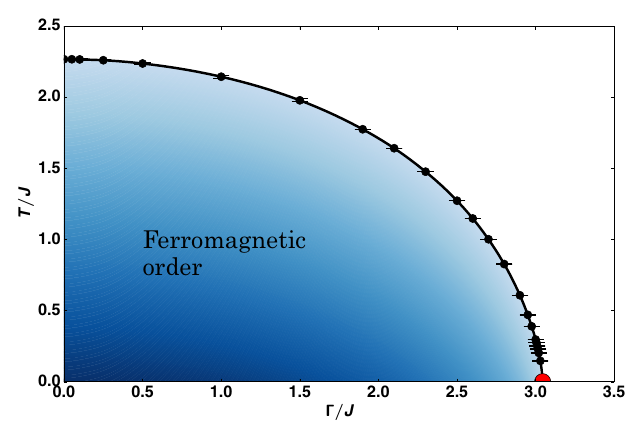
\includegraphics[width=\textwidth]{Figuren/phsyics/2disingphase.png}
    \caption{Phase diagram for 2D transversal Ising model. Figure taken from \cite{Hesselmann2016}}
    \label{2dtisingphasediag}
\end{figure}

\subsection{Heisenberg}

The heisenberg model is given by:

\begin{equation}
    \hat{H} =  -\left( \sum_{<i j>} J_x \sigma^z_i \sigma^z_j + J_y \sigma^y_i \sigma^y_j+ J_z \sigma^z_i \sigma^z_j + h \sum_i \sigma^z_i \right )
\end{equation}

These models have different names depending on the values of $J_{\alpha} $ with $\alpha=x,y,z$. $J_x = J_y \neq J_z = \Delta$ is called the XXZ model.

\subsection{Random}
It's also possible to construct random hamiltonians. \todo{in basis: hermitian H}

\section{Criticality}
\subsection{Phases of matter}

An important area of research is the study of the different phases of (quantum) matter. A phase is a state
of matter in which the macroscopic physical properties of the substance are uniform on a macroscopic length scale. These phase can be measured by thermodynamic function, i.e. by function of a few macroscopic parameters. \cite{Nishimori2011}. More precisely, for a given phase the properties vary as an analytic function of the macroscopic variables.

Interesting physics happens at the boundary between 2 or more distinc phases. The phase transitions were classified by Ehrenfest \cite{Jaeger1998}, who looked at the free energy across the phase boundary. If the free energy shows a discontinuity, it is called first order (or discontinuous) phase transition. Similarly, if the derivitive shows a discontinuity, it is called second order (or continuous). Higher order phase transitions are possible, and there are even examples of infinite order transitions, such as the BKT transition.

\subsection{symmetry breaking}

Sometimes, but not always, a phase transition is  related to spontaneous symmetry breaking. A state $\ket{\Psi}$ is said to be symmetric under a unitary transformation U if the state only changes by a phase factor: $ \hat{U} \ket{\Psi} = e^{i \phi} \ket{\Psi} $. A hamiltonian posesses a symmetry if it commutes with U: $ [H,U]=0$  \cite{Beekman2019}. A remarkable fact is that many ground states are not invariant under a symmetry U of the hamiltonian.

For phase transitions associated with a broken symmetry, one can define an order parameter. This parameter evalutes to 0 for the symmetric phase, but not for the sponteous broken phase.

In continuous or second-order phase transitions the order parameter increases continuously from zero as the critical temperature is traversed. The entropy also changes continuously. On the other hand, the correlation length and related energy scales diverge at the critical temperature. In fact, at the critical temperature of a second-order phase transition, scale invariance systems become scale-invariant, in the sense that physical properties no longer depend on the length (or energy) scale at which they are probed. Many symmetry-breaking phase transitions are second-order, with the onsets of superfluidity, (anti)ferromagnetism and many phases of liquid crystals as famous examples.\cite{Beekman2019}

\subsection{Universality}

Universality looks at the behaviour of the system near a continuous phase transition. These can be discribed well by so called power laws. For classical phase transitions (driven by temperature) near critical temperature $T_c$, observables $a_i$ depend in the following way on the reduced temperature $t=\frac{T-T_c}{T_c}$: $ a_i(t) \sim t^{\alpha_i}$. One would expect that the set of critical exponents ${\alpha_i}$ depends on the precise form of the hamiltonian of the system, but it turns out these exponents can be captured by a limited numer of universality classes. This means that the physics near criticality is completely understood once it is understood for one member of the class.

\subsection{Critical exponents for spin systems}
The following table defines some of the critical exponents for the Ising system.

\begin{table}[h!]
    \centering
    \begin{tabular}{c c c c}
        Symbol & name                \\
        \hline
        m      & magnetisation       \\
        $\xi$  & correlation length  \\
        g      & external field      \\
        t      & reduced temperature \\
        d      & dimension           \\
    \end{tabular}
\end{table}

The 2 point correlation function is defined as $ f( x,y) =  \left < m(x) m(y) \right > -  \left<m(x) \right> \left<m(y) \right> $. At larger distances this decays exponentially fast (see \cref{crt:cft} ) $ f(  x,y ) = e^{ -\frac{ |x-y|}{ \xi} } $, where $\xi$ is the correlation length.

for the ordered phase, the following relations hold: $m ~ |t|^{\beta} $ , $\xi(t) \approx |t|^{-\nu} $. At the critical temperature near a quantum phase transition  $ m \approx |g-g_c|^{\frac{1}{\delta}} $.

\subsection{Finite size scaling}\label{subsec:fss}

Phase transitions only occur for systems with an infinite number degrees of freedom. This poses a problem, as in for instance Monte Carlo simulations only finite grids can be simulated. One computational expensive way to extract the properties in the thermodynamic limit is by making the grid increasingly bigger untill the properties have converged. Fisher's insight was that the properties could also be extrapolated from different finite size calculations by making the following assumption: near a critical point, every thermodynamic properties scales as an universal function of $L/\xi$, with L the size of the system and $\xi$ the correlation length.

Define $t=\frac{T-T_c}{T_c}$. The mathematical formulation is as follows:
\begin{equation}\label{eq:fssansatz}
    A(T,L) = L^{\kappa / \nu} f_A( t L ^{1/ \nu} )
\end{equation}
This holds for t small (near critical point) and L sufficient large compared to the lattice spacing. The exponents can be fitted by plotting $A(T,L)  L^{-\kappa / \nu} $ as a function of $t L ^{1/ \nu}$ for different sizes L and temperature t. For the correct critical exponents and critical temperature, all the points should collapse to one single graph.

From the ansatz \cref{eq:fssansatz}, other ways can be derived to determine certain coefficients.

\subsubsection{Finite size scaling for MPS}

The finite size scaling for MPS is somewhat different. In \cite{Vanhecke2019}, it is argued that $\delta$ can take the place of $1/L$.

Suppose $\lambda_i$ are the eigenvalues of \cref{vumps_transfer_eigs} order from largest real part to smallest. Then
\begin{equation}
    \epsilon_i = - \log( \left | \lambda_i  \right |  )
\end{equation}
Then
\begin{equation}
    \delta = - \sum_i c_i \epsilon_i
\end{equation}
The intuition behind this is as follows: for a MPS approximation, the gaps in the transfer spectrum go always to zero for sufficient large bond dimension. The distance between these gaps is thus a measure for the system size.

\subsubsection{subleading corrections}
In \cite{Beach2005}, it is argued that the form proposed in \cref{eq:fssansatz} does also not fully take into account the finite size effects. Subleading correction could be introduced as follows:
\begin{equation}
    A(T,L) = L^{\kappa / \nu} ( 1+c L^{-\omega} ) f_A( t L ^{1/ \nu} -d L^{-phi/nu} )
\end{equation}
Indeed, this reduces to \cref{eq:fssansatz} for sufficient large L. Because there is always data need around the critical point, the original procedure could be biased and result in wrong parameters. On the other hand, introducing extra parameters can lead to overfitting, again not improving the result.

\subsection{CFT}\label{crit:cft}

\todo{central charge}

\subsection{Quantum phase transitions}

A traditional 2nd order phase transition is driven by a change in temperature. Quantum phase transitions on the other hand happen at zero temperature under influence of another parameter g of the model. At finite temperature, 2 things can happen: either there is a line connecting a classical 2nd order phase transition to the quantum phase transition, or the phase transition disappears at finite temperature \cite{Sachdev1999}.

\begin{figure}
    \center
    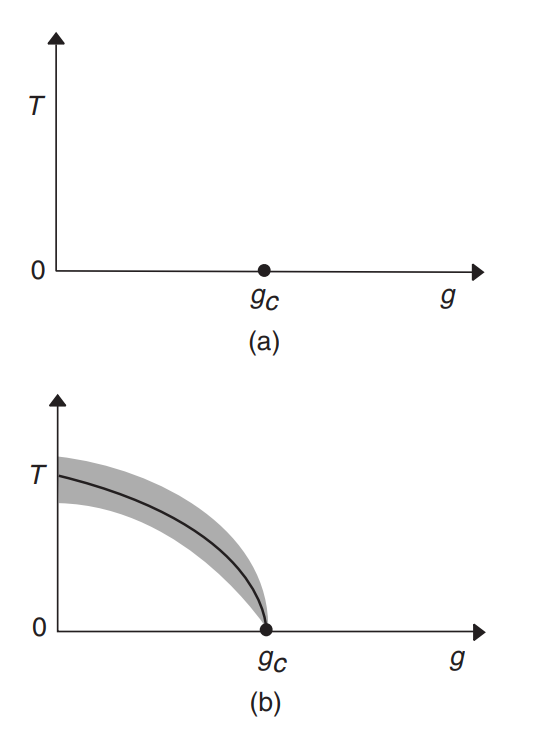
\includegraphics[width=0.5\textwidth]{Figuren/crit/Screenshot from 2021-05-06 15-58-55.png}
    \caption{ Two possible phase diagrams of a system near a quantum phase transition. In both cases there is a quantum critical point at $g = g_c$ and $T = 0$ . In (b), there is a line of $T > 0$ second-order phase transitions terminating at the quantum critical point. The theory of phase transitions in classical systems driven by thermal fluctuations can be applied within the shaded region of (b).  Figure and caption taken from \cite{Sachdev1999}. }
    \label{fig:crit:qtran}
\end{figure}

\subsection{Quantum to classical mapping}

\todo{Quantum to classical mapping}

\section{Benchmarking}
\subsection{dioganalsation}

The performance of the MPO construction can be compared with the exact diagonalisation of the hamiltonian for a given number of sites. To obtain a faithful results, the number of sites should be as high as possible. In practice, diagonalisation of large matrices becomes slow and memory consuming. The size grows exponentially in the number of sites: $d^{n} \times d^{n} $. A double takes 8 bytes of memory.A Rough estimated of the amount of RAM $R$ needed to store this complex array is:

\begin{equation}
    R = d^{2 n} \times 16 bytes
\end{equation}

Which means a 14 site chain already takes up  GB of RAM.

\todo{time complexity algoritms}

\todo{open chain or cyclical}


\subsubsection{norms}

\todo{trace norm, schatten p norm, ...}

The schatten 2 norm is used in the following analysis, dentoted by ${\| \cdot \|} _{2}$. In the figures the relative error $\epsilon$ is reported.


\def \expHBlock {\expH{4}{ $e^{- \beta \hat{H}_{n}}$   }{ {,,"...",} }{ {,,"...",} }{}{} }
\def \Mn {\mpo{4}{ {0,,,,0}  }{}{}{{0,0,1,0,0}}{}}


\begin{equation}
    \epsilon = \frac{  {  \left \|  \expHBlock - \Mn  \right \|} _{2}  }{ {  \left\|  \expHBlock \right \|}_2}
\end{equation}


\subsubsection{Ising}

The first model used to benchmark the different types of MPO's is the transversal ising model. For type A the $\epsilon$ increases with
$\beta$. As expected, the relative error decreases with increasing order.

The behaviour of type B is more chaotic. The error increases no longer monotonously. For small values of $\beta$, the order is truncated.


\begin{figure}[H]
    \center
    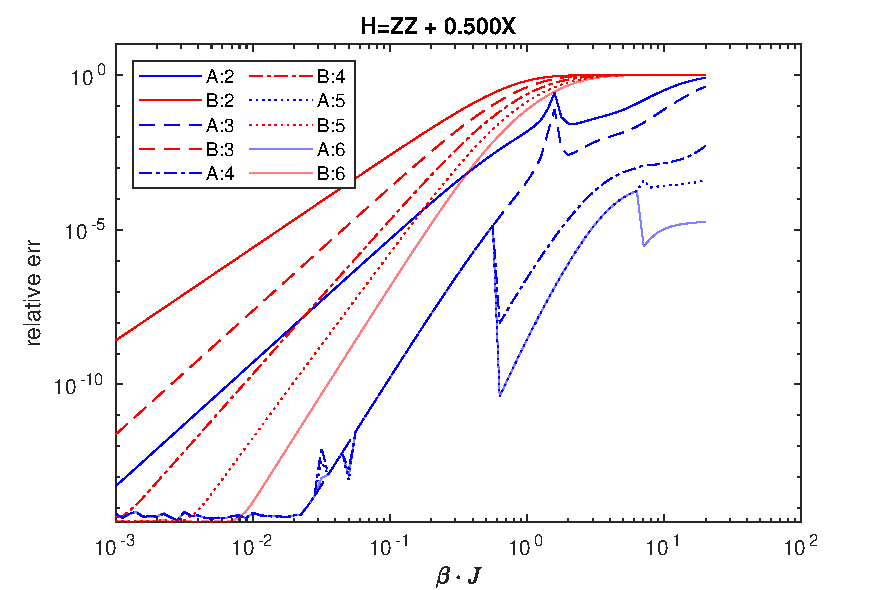
\includegraphics[width=\textwidth]{Figuren/benchmarking/t_ising_copmAB6.pdf}
    \caption{Comparison type A and B for Transversal Ising}
    \label{fig:benchmark:tising}
\end{figure}

\subsubsection{Heisenberg}

For the Heisenberg model, type A is also an improvement over type B. For large values of $\beta$, type A is not able to reproduce the exact


\begin{figure}[H]
    \center
    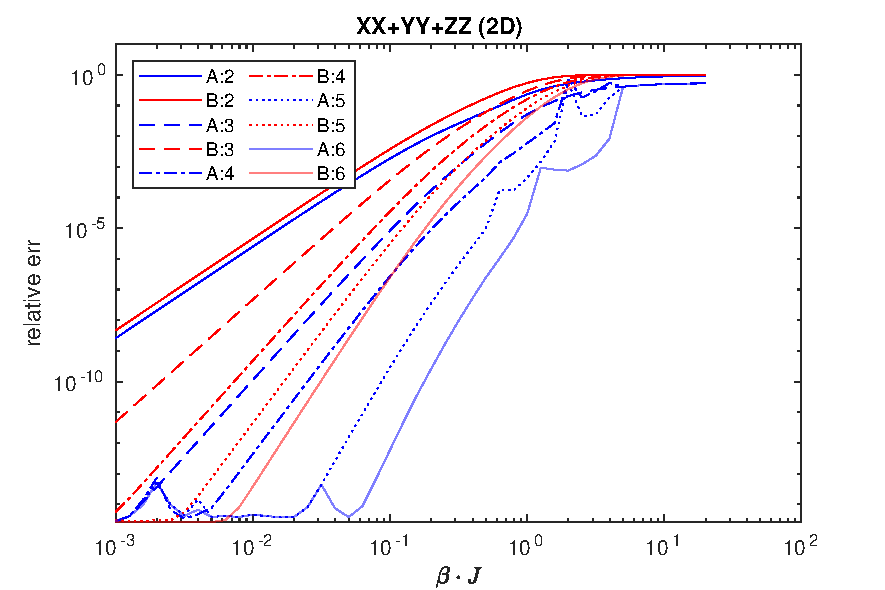
\includegraphics[width=\textwidth]{Figuren/benchmarking/heisenberg_compAB6.pdf}
    \caption{Comparison type A and B for Heisenberg}
    \label{fig:benchmark:Heisenberg}
\end{figure}


\todo{run with M=11}

\subsection{Random}

To give a representative overview for random hamiltonians, several simulations were run. The single site and nearest neighbourgh hamiltonians are generated by making hermitian matrices with random real and complex numbers between -1 and 1. In order to compare the different graphs, the engergy scale is set such that the norm of the 2 site hamiltonian is 1.


Clearly, the performance of type B is almost independent on the chosen random variables. For type A there is more variation. Sometimes there are spikes for a given $\beta$. Despite the worse relative error, higher orders (with exact the same lower order blocks) seem to remove the spike.

For most of the trials, orders higher than 6 get truncated.

\begin{figure}[H]
    \begin{subfigure}[]{\textwidth}
        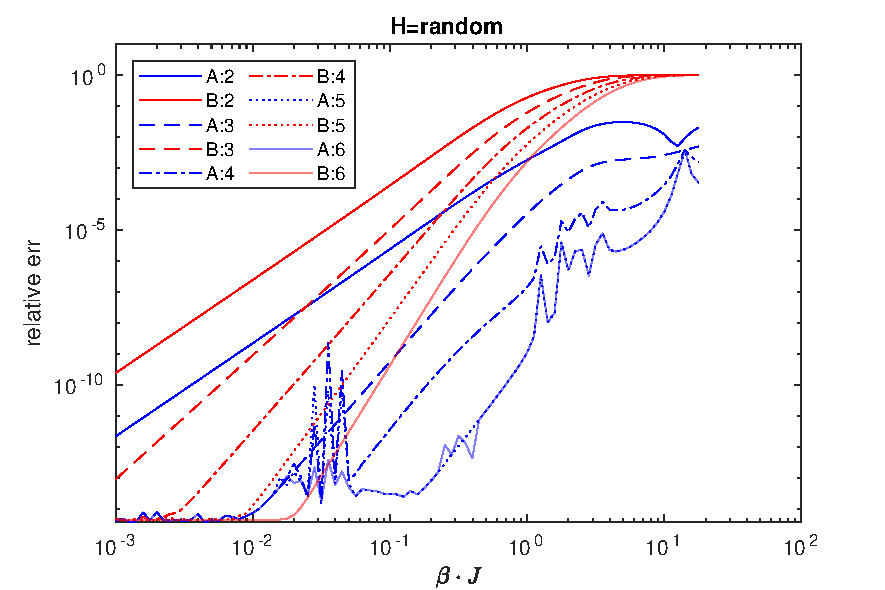
\includegraphics[width=\textwidth]{Figuren/benchmarking/random_copmAB6.pdf}
        \subcaption{test}
    \end{subfigure}

    \medskip

    \begin{subfigure}[]{\textwidth}
        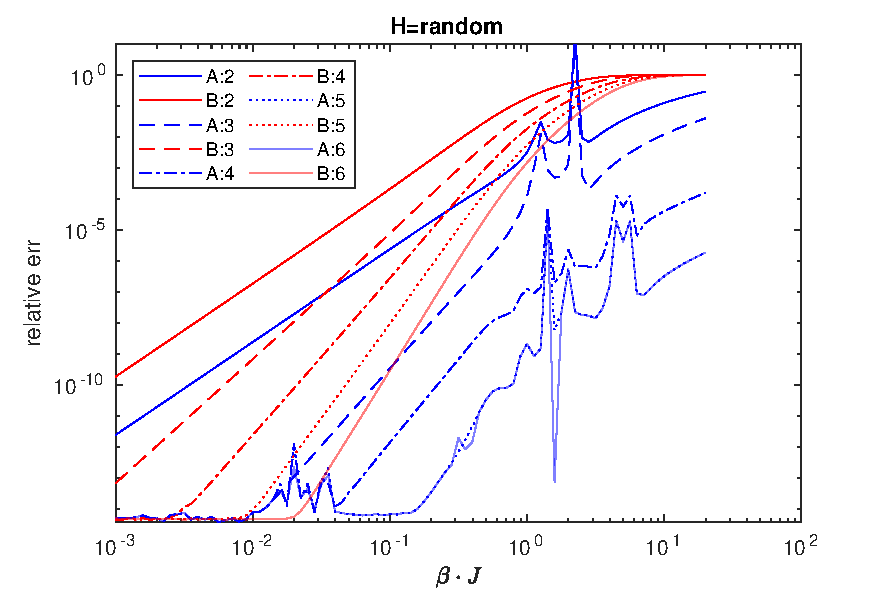
\includegraphics[width=\textwidth]{Figuren/benchmarking/random_copmAB6_2.pdf}
        \subcaption{test}
    \end{subfigure}

    \caption{test }
\end{figure}

\begin{figure}[H]\ContinuedFloat
    \begin{subfigure}[]{\textwidth}
        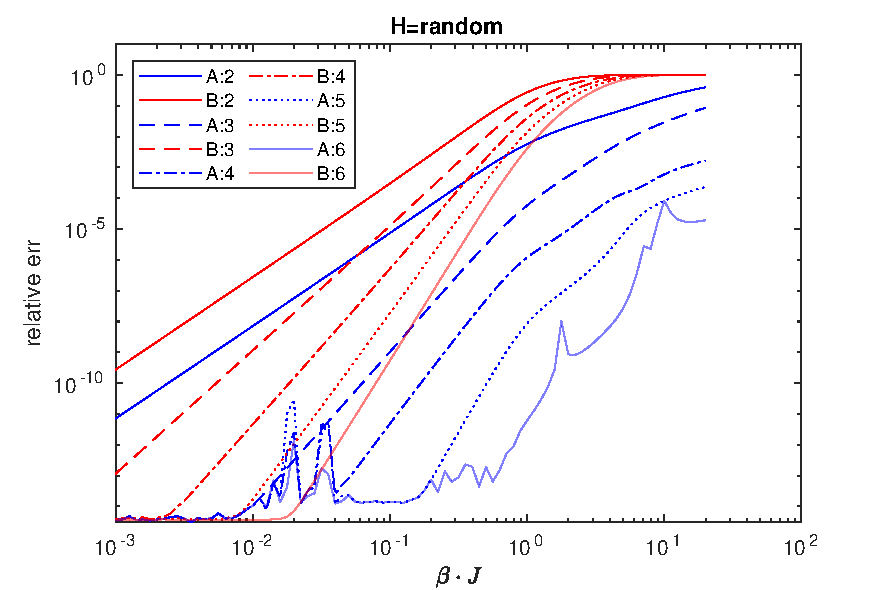
\includegraphics[width=\textwidth]{Figuren/benchmarking/random_copmAB6_3.pdf}
        \subcaption{test}
    \end{subfigure}

    \begin{subfigure}[]{\textwidth}
        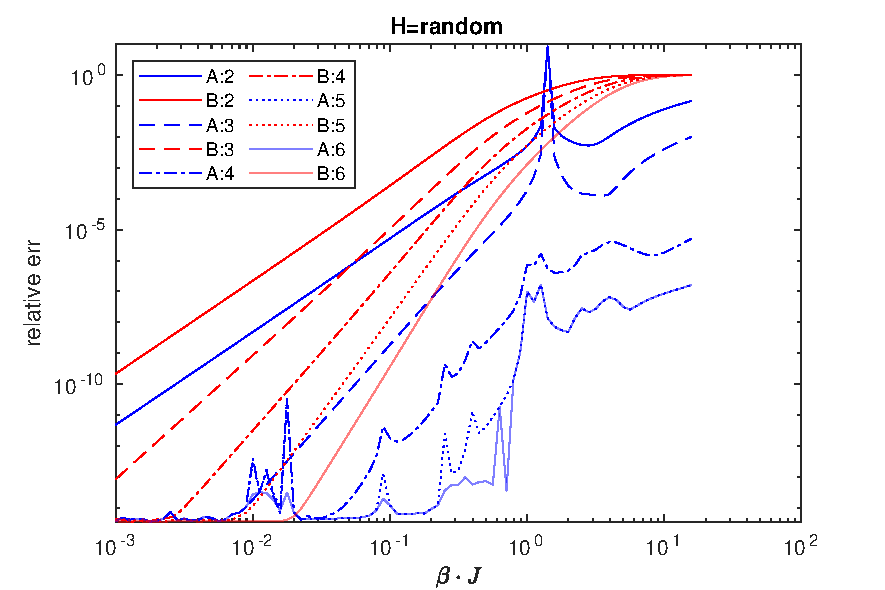
\includegraphics[width=\textwidth]{Figuren/benchmarking/random_copmAB6_4.pdf}
        \subcaption{test}
    \end{subfigure}
    \caption{test (cont.) }
    \label{fig:benchmark:Random}
\end{figure}


\subsection{analytical results}

\bibliographystyle{elsarticle-num}
\bibliography{bib}
\end{document}
